\documentclass[10pt,a4paper]{article}
\usepackage[latin1]{inputenc}
\usepackage{amsmath}
\usepackage{amsfonts}
\usepackage{amssymb}
\usepackage[]{theorem}
\usepackage[nottoc]{tocbibind}
\usepackage[hidelinks]{hyperref}
\usepackage{appendix}
\usepackage{listings}
  %\usepackage{minitoc}
\usepackage{graphicx}
\usepackage{float}
\usepackage{makecell}
\usepackage{authblk}
\usepackage[bottom]{footmisc}


\setlength{\topmargin}{-.5in}
\setlength{\textheight}{9in}
\setlength{\oddsidemargin}{.125in}
\setlength{\textwidth}{6.25in}

\newcommand {\subsubsubsection} [1] {\vskip 0.5em {\bf \em #1}}

%\newcommand {\comm} [1] {}
\newcommand {\comm} [1]
{
\par
\setlength{\leftskip}{-0.8in}
\begin{tabular} {p{0.1cm} | p{\textwidth}}
  {\bf ?} & {#1}
\end{tabular}
\par
\setlength{\leftskip}{0in}
}


\newcommand {\cond} {, & \textrm{if }}
\newcommand {\otherwise} {, & \textrm{else}}

\newcommand {\Forall} {\forall \ }
\newcommand {\eqdef} {\triangleq}
\newcommand {\equivalent} {\Leftrightarrow}
\renewcommand {\implies} {\Rightarrow}
\renewcommand {\impliedby} {\Leftarrow}
\renewcommand {\And}  {\ \& \ }
\newcommand {\Or}  {\ \vee \ }
\newcommand {\QED} {$\square$ \ \par }
\newcommand {\proofword}  {{\par \sf Proof:\ }}
\newcommand {\proof} [1] {\proofword #1 \QED \par}
\newcommand {\definition} [2] {\bigskip {\bf Definition} {\rm \sc #1} \par #2 \QED \bigskip}
\newcommand {\example} [2] {\bigskip {\bf Example.} {#1} \par #2 \QED}
\newcommand {\theorem} [2] {\bigskip {\bf Theorem} {\rm \sc #1} \par #2 \QED \bigskip}
\newcommand {\ve} {\mathbf}
\newcommand {\vecc} {\boldsymbol}
\newcommand {\Questions} {\vspace{5mm} {\bf Unresolved Questions:}}
\newcommand {\assert} {\square \ }

\renewcommand {\P} {\mathrm P}
\newcommand {\E} {\mathrm E \ }
\newcommand {\var} {\mathrm {var} \ }
\newcommand {\cov} {\mathrm {cov} }
\newcommand {\cor} {\mathrm {cor} }
\newcommand {\N} {\mathbb N}
\newcommand {\Z} {\mathrm Z}
\newcommand {\R} {\mathbb R}
\newcommand {\C} {\mathbb C}
\newcommand {\I} {\mathbb I}
\newcommand {\supp} {\mathrm {Supp}}
\newcommand {\mat} {\mathrm}
\newcommand {\trc} {\mathrm {tr} \ }
\newcommand {\VC} {\mathrm {VC} }
\newcommand {\const} {\mathrm {const} }
\newcommand {\sgn} {\mathrm {sgn} }
\newcommand {\dom} {\mathrm {dom} }
\newcommand {\range} {\mathrm {range} }
\newcommand {\Arg} {\mathrm {Arg} \ }

\newcommand {\LCA} {\mathrm {LCA} }  % least common ancestor (in a tree)

\newcommand {\nul} {\mathrm {null}}
\newcommand {\Dt} {\Delta t}
\newcommand {\PC} {\mathrm {PC} }
\newcommand {\MDS} {\mathrm {MDS} }
\newcommand {\CC} {\mathrm {CC} }

\newcommand {\re} {\mathrm {re}}
\newcommand {\cl} {\mathrm {cl}}
\newcommand {\intr} {\mathrm {int}}

\newcommand {\<} {\langle}
\renewcommand {\>} {\rangle}

\newcommand {\dotve} [1] {\dot {\ve #1}}

\newcommand {\la} [1] {\lambda (#1) \ }

\newcommand {\lhs} {\mathrm {lhs}}
\newcommand {\rhs} {\mathrm {rhs}}

\providecommand{\keywords}[1]
{
  \small
  \textbf{\textit{Keywords---}} #1
}

\makeatletter
\DeclareRobustCommand{\cev}[1]{%
  {\mathpalette\do@cev{#1}}%
}
\newcommand{\do@cev}[2]{%
  \vbox{\offinterlineskip
    \sbox\z@{$\m@th#1 x$}%
    \ialign{##\cr
      \hidewidth\reflectbox{$\m@th#1\vec{}\mkern4mu$}\hidewidth\cr
      \noalign{\kern-\ht\z@}
      $\m@th#1#2$\cr
    }%
  }%
}
\makeatother



\providecommand{\keywords}[1]
{
  \small
  \textbf{\textit{Keywords---}} #1
}


\title{Building Large Phylogenetic Trees in Log-Linear Time}
\author[1]{Slava Brover\footnote{E-mail: brovervv@ncbi.nlm.nih.gov}}
\affil[1]{\small National Center for Biotechnology Information, National Library of Medicine, National Institutes of Health, Bethesda, MD 20894, USA.}


\begin{document}
\maketitle

\begin{abstract}
A practical scalable algorithm to build large phylogenetic trees is described.
The trees are based on dissimilarities between objects
and use the least squares optimization criterion.
Tree leaves and arcs have fitting criteria as the measures of correctness.
The main idea of fast tree optimization is to extract subgraphs out of the whole tree, optimize them as separate small trees and then embed them back into the whole tree.
A large tree is built by inserting new objects into an existing tree and optimizing the whole tree incrementally.
Dissimilarities are not computed for all pairs of objects, but for the pairs chosen by the algorithm preferring pairs closer in the tree.
Different types of object outliers are identified and removed from the tree.
The running time of the incremental tree building is $O(n \log^4 n)$ and space is $O(n \log^3 n)$, where $n$ is the number of objects.
The software is provided at {\tt github}.
The global phylogenetic trees of GenBank bacteria, fungi, protist genomes, and prokaryotic 16S rRNA and fungal ITS rRNA are provided.
\end{abstract}

\keywords {Phylogeny, Distance tree, Least squares, Phylogenetic placement, Bacteria, Fungi, Protists, 16S rRNA, ITS rRNA.}

%\dominitoc
\tableofcontents



\section {Introduction}

When a phylogenetic tree of genomes or rRNA sequences of a given taxonomic group is built,
usually the tree building is preceded by the selection of representative genomes or sequences.
But it may be important to build a phylogenetic tree for all available genomes or rRNA sequences.
Such a tree will be referred to as a {\em global} phylogenetic tree.

A global phylogenetic tree can be used:
\begin{itemize}
  \item to verify the correctness of taxonomic assignment of genomes or rRNA sequences, especially of type strains;
  \item to select representative genomes at a given level of granularity;
  \item to identify outbreaks in epidemiological data;
 %\item to estimate the evolutionary relation between organisms in the gray zone between defined taxa;
  \item to quickly produce trees for any desired subsets of objects by removing all extra objects for pilot studies;
  \item to quickly find genomes close to a specific genome.
\end{itemize}

Since there is no publicly available tool to build a global phylogenetic tree for, say, all GenBank bacterial genomes,
it was undertaken to create such a tool.

The optimization criterion of a global tree was chosen to be the least squares distance criterion because
\begin{itemize}
  \item the current MLE phylogenetic methods are computationally intensive and cannot compare genomes above and below species level in the same data set;
  \item the minimum evolution method is not a maximum likelihood method in the statistical sense.
\end{itemize}

The currently available least squares distance tools PHYLIP~\cite{Phylip} and PAUP~\cite{PAUP} are too slow even for small trees.
Therefore, a new tool, {\tt makeDistTree}, was created for fast building of small phylogenetic trees,
and a system of tools with the main script {\tt distTree\_inc.sh} was created to build a phylogenetic tree
for a large set of genomes or rRNA sequences using the dissimilarities between them.

By the least squares optimization criterion,
the tree topology and arc lengths of the tree are optimized so that the tree distances should fit the dissimilarities.
A weighted least squares criterion is used as the fitness measure.

Genomes may not fit the tree well due to being hybrid, contaminated or due to sequencing problems.
They are identified as outliers and removed from the tree.

The main problem with building a distance tree for a large set of genomes or sequences is that
computing all pairwise dissimilarities is not feasible.
This problem is solved by building an initial tree only for a subset of genomes or sequences with a complete dissimilarity matrix,
and then iteratively incrementing and optimizing the tree,
where the dissimilarities are not computed for all pairs of genomes or sequences,
but for the pairs chosen by the algorithm.
The achieved running time of this algorithm is log-linear.

The incremental algorithm allows fast adding of new genomes or sequences to an existing tree.

The provided tools allow building and maintaining a phylogenetic tree, for example, for all {\it Escherichia coli} genomes in a hospital database
where the number of genomes is of the order of hundreds thousands.

This paper describes the algorithms used for the incremental distance tree building.

Examples of large distance trees which have been built for major microbial applications at the kingdom taxonomic level and above are provided.

%\comm{Big data - less quality for small trees, but compensated by the quantity of data for large trees.}


\section {Basic definitions}

The constants defined in this Section will used in the whole paper.
The constants introduced in the next Sections will be used only in those Sections.

Let~$S$ be a set of {\em objects}.
Each object has a unique name.

$$ n = |S|.$$


\subsection{Dissimilarity}
\label{sec:Dissim}

Let $d:S,S \to \R$ be a {\em dissimilarity} function,
which may not be defined for all pairs of objects.
It is required that $d_{xy} = d_{yx}$ and $d_{xx} = 0$.

$$ P = \{\{x,y\} : x \in S \And y \ \in S \And x \ne y \And d_{xy} \textrm{ is defined}\}. $$
$$ p = |P|. $$

Objects~$x$ and~$y$ having $d_{xy} \le 0$ are {\em indiscernible}, otherwise they are {\em discernible}.
Negative dissimilarities can be between interior tree nodes, see Section~\ref{sec:optimizeSubgraph}.
The {\em indiscernibility relation} is
$$\{\{x,y\} \subseteq P : d_{xy} \le 0\}. $$
Its transitive closure is an equivalence relation.
Let~$\mathfrak I$ be the set of equivalence classes of this equivalence relation.

The {\em neighbors} of an object $x \in S$ are the objects of~$S$ having a dissimilarity with~$x$:
$$ N(x) = \{y \in S : \{x,y\} \in P \}.$$

$$ \sum_{x \in S} |N(x)| = 2 p. $$
$$ \textrm{mean } \{|N(x)| : x \in S \} = 2 \ p / n. $$

A {\em hybrid triangle} is a triple of objects~$c$, $p_1$ and~$p_2$ for which the triangle inequality is violated:
$$ h = \frac {d_{p_1 p_2}} {d_{p_1 c} + d_{p_2 c}} > 1. $$
The object~$c$ is the hybrid triangle {\em child},
and the objects~$p_1$ and~$p_2$ are the hybrid triangle {\em parents}.
The value~$h$ is the {\em hybridness} of the hybrid triangle.
The child and parents of a specific hybrid triangle~$tr$ are indicated by~$tr.c$, $tr.p_1$ and~$tr.p_2$.
A non-empty subset of the objects of a hybrid triangle~$tr$ is the set of {\em hybrid triangle outliers} denoted by~$H(tr)$.
%and the set of the rest objects of a hybrid triangle~$tr$ is denoted by~$\overline H(tr)$.

Let~$\mathfrak T$ be a set of hybrid triangles.
For $tr \in \mathfrak T$
\begin{align*}
Tr_c(tr)     &= \{x \in \mathfrak T : x.p_1 = tr.p_1, x.p_2 = tr.p_2 \}, \\
Tr_{p_1}(tr) &= \{x \in \mathfrak T : x.c = tr.c, x.p_2 = tr.p_2 \}, \\
Tr_{p_2}(tr) &= \{x \in \mathfrak T : x.c = tr.c, x.p_1 = tr.p_1 \}.
\end{align*}
%$$ H(\mathfrak T) = \bigcup_{tr \in \mathfrak T} H(tr). $$


\subsection{Tree}
\label{sec:tree}

An {\em undirected tree}~$T$ is a connected undirected graph with no cycles.

A {\em directed tree} is an undirected tree where one of the nodes is a {\em root}, and all arcs are directed to the root.
In the sequel a directed tree will be referred to as a {\em tree}.

For a directed arc~$(x,y)$, node~$y$ is the {\em parent} of node~$x$, and node~$x$ is a {\em child} of node~$y$, and the arc is directed from~$x$ to~$y$:
$$ y = parent(x). $$
$$ x \in Children(y). $$
The node $parent(root)$ does not exist.

$$ Descendants(x) = \{x\} \cup \bigcup_{z \in Children(x)} Descendants(z). $$
$$ Ancestors(x) = \{x\} \cup
  \begin{cases}
    \emptyset, &\text{ if } x = root,\\
    Ancestors(parent(x)), &\text{ else}.
  \end{cases}
$$

The nodes with degree~1 are {\em leaves}, denoted by $Leaves(T)$,
and the other nodes of~$T$ are {\em interior} nodes.

$Path(x,y)$ is the set of arcs on the unique undirected path from node~$x$ to node~$y$.

Arcs~$j$ are assigned the {\em length}~$l_j > 0$.

The {\em tree distance} between nodes~$x$ and~$y$
$$ l_{xy} = \sum_{j \in Path(x,y)} l_j. $$
The tree distance satisfies the distance axioms.

The {\em topology} of a tree is the interior nodes and the arcs of the tree, disregarding arc lengths.

A connected subgraph of a tree is a tree.

The {\em boundary} of a connected tree subgraph~$A$, denoted by $Boundary(A)$,
is a subset $B \subseteq A$ such that all nodes in~$B$ have degree~1 in~$A$.

The nodes of the tree centered at node~$x$ with radius~$k$
$$ Area(x,k) = \{y : |Path(x,y)| \le k\}. $$
The nodes of~$Area(x,k)$ make up a connected subgraph.
$$ Boundary(x,k) = Boundary(Area(x,k)). $$

$$ depth(x) = |Path(x,root)|. $$
$$ height(x) = \max_{y \in Descendants(x)} |Path(x,y)|. $$

%The {\em least common ancestor} of nodes~$x$ and~$y$
%$$ lca(x,y) = \arg \min_{z \in Ancestors(x) \cap Ancestors(y)} depth(z). $$

At each arc~$j$ the list of object pairs~$\{x,y\}$ is stored:
$$ Pairs(j) = \{\{x,y\} \in P : j \in Path(x,y)\}. $$
If~$x$ is a leaf then
$$ Pairs(x,parent(x)) = \{(x,y) : y \in N(x) \}. $$
$$ \sum_{j \textrm{ is a leaf arc}} |Pairs(j)| = 2 \ p. $$

A {\em genogroup} of {\em barrier~$\beta$} is a minimal subset~$G$ of~$S$ such that
$$ \forall x \in G \ \forall y \in S : (l_{xy} \le \beta \implies y \in G). $$
All genogroups of the same barrier make up a partition of~$S$.


\section {Assumptions}
\label{sec:assum}

\begin{enumerate}
  \item All nodes of a tree have degree~1 or at least~$3$, except the root.
  The root can have degree~2.

  \item The degree of an interior node is at most~500.
        Practically it is close to~3, but can be higher if interior arcs are deleted in the middle of optimization.

  \item $height(root)$ is $O(\log n)$.
   In other words, the tree should be balanced.
   This holds for evolutionary data with molecular clock.

 %\item $\forall x \in S : l_{root,x} = \Theta(1)$ which is true for evolutionary data with molecular clock.

  \item The computation of dissimilarities is an external process relative to the provided tools.
        It is required that the computation of~$d_{xy}$ should have time~$O(1)$.
        The dissimilarities used in this paper satisfy this requirement, see Appendix~\ref{app:data}.

  \item The number of objects~$n$ is bounded by a very large number: $\log \log n = O(1)$.

  \item Allocating memory of~$p$ bits and setting all bits to~0 takes time~$O(1)$.
    \label{asmp_alloc}
\end{enumerate}

Consequences from the assumptions:
\begin{itemize}
  \item The number of the nodes of the tree is~$O(n)$
        and the number of the arcs is~$O(n)$.

  \item For a constant~$k$, $|Area(x,k)| = O(1)$.
  \item The time to compute $Path(x,y)$ is $O(\log n)$ and $|Path(x,y)| = O(\log n)$.
  \item The cumulative time to compute $Pairs(j)$ is~$O(p \log n)$.
  \begin{equation} \label{eq:Pairs}
     \sum_{j \textrm{ is not a leaf arc}} |Pairs(j)| = O(p \log n).
  \end{equation}
  Average $|Pairs(j)|$ is~$O(p/n \log n)$.
\end{itemize}


\section {Least squares model}

\subsection {Model and criterion}

A {\em tree model} of a dissimilarity~$d$ is defined as a tree~$T$, such that $Leaves(T) = S$.

The {\em absolute criterion} of a tree model is the weighted least squares fitness function defined as
$$ |\ve \epsilon|^2 = \sum_{\{x,y\}  \in P} w_{xy} \ (d_{xy} - l_{xy})^2, $$
where the {\em weights} are defined as
\begin{equation} \label{eq:weight}
w_{xy} = \frac 1 {v(l_{xy})},
\end{equation}
which is a classic approach, see~\cite{Felsenstein}.
The value~$v(l)$ is the {\em dissimilarity variance}, see Section~\ref{sec:dissimVar}.

The {\em relative criterion} is defined as
$$ \sqrt {\frac {|\ve \epsilon|^2} {\sum_{\{x,y\} \in P} w_{xy} \ d_{xy}^2}}. $$

The absolute criterion depends on the dissimilarity measurement scale,
whereas the relative criterion does not.
The relative criterion is between~0 and~1:

If the dissimilarities~$d_{xy}$ are the realizations of independent random variables
\begin{equation} \label{eq:model}
  D_{xy} \sim Normal \ (l_{xy}, \alpha \ v(l_{xy}))
\end{equation}
for $\alpha > 0$,
then the likelihood maximization is equivalent to the minimization of
  $$  \frac {|\ve \epsilon|^2} \alpha + \sum_{\{x,y\} \in P} \ln v(l_{xy}) + p \ln \alpha, $$
which is minimized at
$$ \alpha = \frac {|\ve \epsilon|^2} p, $$
and, therefore, is equivalent to the minimization of
\begin{equation} \label{eq:MLE_crit}
  \ln \frac {|\ve \epsilon|^2} p + \frac 1 p \sum_{\{x,y\} \in P} \ln v(l_{xy}).
\end{equation}

Criterion~(\ref{eq:MLE_crit}) is minimized approximately
by iteratively computing weights and minimizing the absolute criterion.

If the variances of~$D_{xy}$ are too large, which is often the case with RNAs,
then~$v(d_{xy})$ can be used instead of~$v(l_{xy})$ in~(\ref{eq:weight})
as better estimates of the dissimilarity variances.
In this case the minimization of the absolute criterion is equivalent to the likelihood maximization.

Given~(\ref{eq:model}),
$$ \forall \ \{x,y\} \in P : w_{xy} \ (d_{xy} - l_{xy})^2 \sim \alpha \ \chi^2(1). $$



\subsection{Object and arc criteria}

The absolute criterion can be split per object or arc,
and normalized object or arc criteria can be defined based on their distributions.
This allows computing the outlier $p$-values
and the degrees of certainty
of leaves and arcs in the tree.

The {\em absolute object criterion} of object~$x$ are the components of $|\ve \epsilon|^2$ involving only the object~$x$:
$$ |\ve \epsilon_x|^2 = \sum_{y \in N(x)} w_{xy} \ (d_{xy} - l_{xy})^2. $$
$$ \sum_{x \in S} |\ve \epsilon_x|^2 = 2 |\ve \epsilon|^2. $$

Since $\var \chi^2(1) = 2$,
the {\em normalized object criterion} of object~$x$
%$$ \frac {|\ve \epsilon_x|^2 \ / \ |N(x)|} {|\ve \epsilon|^2 / p} $$
$$ \frac {|\ve \epsilon_x|^2 / \alpha - |N(x)|} {\sqrt {2 \ |N(x)|}} \sim Normal(0,1) $$
for $|N(x)| \ll p$ and large~$p$,
where the value~$\alpha$ is a parameter of the probabilistic model~(\ref{eq:model}).

The {\em deformation} of dissimilarity~$d_{xy}$ is defined as
$$ def(x,y) = \frac {(d_{xy} - l_{xy})^2} {\min(d_{xy},l_{xy})}, $$
which has approximately the same distribution as $w_{xy} \ (d_{xy} - l_{xy})^2$.

The {\em object deformation} of object~$x$ is defined as
$$ def(x) = \max_{y \in N(x)} def(x,y). $$

The {\em relative object deformation} of object~$x$ is defined as
\begin{equation} \label{max_chi2}
 \frac {def(x)} {\textrm{mean } \{def(y,z) : \{y,z\} \in P\}} \sim \max \{Y_i : 1 \le i \le \textrm{mean } \{|N(y)| : y \in S \} \},
\end{equation}
where~$Y_i$ are i.i.d.~random variables distributed as~$\chi^2(1)$.

The {\em absolute arc criterion} of arc~$j$ are the components of $|\ve \epsilon|^2$ involving only the arc~$j$
multiplied by the proportion of $l_j$ in the distances:
$$ |\ve \epsilon_j|^2 = \sum_{\{x,y\} \in Pairs(j)} w_{xy} (d_{xy} - l_{xy})^2 \ \frac {l_j} {l_{xy}}. $$
$$ \sum_{j \in T} |\ve \epsilon_j|^2 = |\epsilon|^2. $$

The {\em absolute arc error density} of arc~$j$ is absolute arc criterion divided by the arc length: $|\ve \epsilon_j|^2 / l_j$.

The {\em normalized arc error density} of arc~$j$ is defined as
$$   \frac {|\ve \epsilon_j|^2 / (\alpha \ l_j) - \sum_{\{x,y\} \in Pairs(j)} 1 / l_{xy}}
           {\sqrt {2 \sum_{\{x,y\} \in Pairs(j)} 1 / l^2_{xy}}}
   = \frac {\sum_{\{x,y\} \in Pairs(j)} (w_{xy} (d_{xy} - l_{xy})^2 / \alpha - 1) / l_{xy}}
           {\sqrt {2 \sum_{\{x,y\} \in Pairs(j)} 1 / l^2_{xy}}}
   \sim Normal(0,1)
$$
for $|Pairs(j)| \ll p$ and large~$p$.


\subsection{Dissimilarity variance}
\label{sec:dissimVar}

An increasing function~$v(l) > 0$, where $l > 0$, is a {\em dissimilarity variance function}.

The dissimilarity variance functions used in the provided tools are in Table~\ref{tab:dissimFunc}:
\begin{table}[H]
  \centering
  \begin{tabular}{|l|c|}
    \hline
    Function name & $v(l)$  \\
    \hline
    Exponential & $e^l$ \\
    Linear-exponential & $e^l-1$ \\
    Power (with parameter~$x$) & $l^x$ \\
    \hline
  \end{tabular}
  \caption{Dissimilarity variance functions}
  \label{tab:dissimFunc}
\end{table}

The linear-exponential function is approximately linear if $l \approx 0$.
Its model is in Appendix~\ref{app:dissimVarLinExp}.

For power dissimilarity variance function
multiplying~$l$ by a positive constant multiplies~$|\ve \epsilon|^2$ by a positive constant,
which preserves the tree topology.
However, for the exponential and linear-exponential dissimilarity variance functions
multiplying~$l$ by a positive constant can change the tree topology.


\subsection{Avoiding zero dissimilarity variance}

For some pairs of objects their dissimilarity variances can be~0, which makes their weights infinite,
and, therefore, $|\ve \epsilon|^2$ infinite.

For indiscernible objects
this occurs always if the dissimilarity variance is $v(d_{xy})$,
and may happen if the dissimilarity variance is $v(l_{xy})$.
Therefore, in this work
the pairs of indiscernible objects are removed from~$P$, and therefore, from~$|\ve \epsilon|^2$,
and for indiscernible objects a fixed topology is created:
for each non-singleton indiscernibility class~$I \in \mathfrak I$ a subtree of depth~1 is created whose set of leaves is~$I$ and whose arcs have length~0.
Then the tree model is optimized only for discernible objects
and
$$ |\ve \epsilon|^2 \ge \sum_{\{x,y\} \in P \ : \ x,y \in I, I \in \mathfrak I} w_{xy} \ d^2_{xy}. $$

If the dissimilarity variance is $v(l_{xy})$,
then each time before the weights~$w_{xy}$ are computed,
the arc of each leaf~$x$ is extended by~$\lambda_x$,
where
$$ \lambda_x =
  \begin{cases}
    0, & \textrm {if } Z_x = \emptyset, \\
    \frac 1 2 \min Z_x, & \textrm {else},
  \end{cases}
$$
$$ Z_x = \{ d_{xy}: \{x,y\} \in P \And l_{xy} = 0 \And d_{xy} > 0 \}. $$
which changes $l_{xy} = 0$ to $0 < l_{xy} \le d_{xy}$.



\section{Tree optimization algorithms}

Finding a globally optimal distance tree model is NP-hard~\cite{NPHard}.

The algorithms in this Section find a locally optimal tree model.

These algorithms allow arcs with zero length.
Such arcs and their child nodes are deleted.


\subsection{Optimization of a connected subgraph}
\label{sec:optimizeSubgraph}
Let~$A$ be a connected subgraph of a tree model~$T$.

Let~$q, r \in Boundary(A)$, such that $q \ne r$.
Let~$T_q$ be the maximal subgraph of~$T$ intersecting with~$A$ in~$\{q\}$,
and
let~$T_r$ be the maximal subgraph of~$T$ intersecting with~$A$ in~$\{r\}$.
The graphs~$T_q$ and~$T_r$ are trees.
Let $Q = Leaves(T_q) \setminus \{q\}$,
and $R = Leaves(T_r) \setminus \{r\}$.
$Q \subseteq S$ and $R \subseteq S$.

Consider the components of the absolute criterion~$|\ve \epsilon|^2$,
where $x \in Q$ and~$y \in R$,
then
$$ d_{xy} - l_{xy} = d_{xy} - (l_{xq} + l_{qr} + l_{ry}) = (d_{xy} - l_{xq} - l_{ry}) - l_{qr}. $$

Let vector $\ve d_{qr}$ indexed by~$x$ and~$y$ be defined as
$$\ve d_{qr}[x,y] = d_{xy} - l_{xq} - l_{ry},$$
then
$$ \sum_{x \in Q, y \in R} w_{xy} \ (d_{xy} - l_{xy})^2
     = \sum_{x \in Q, y \in R} w_{xy} \ (\ve d_{qr}[x,y] - l_{qr})^2
     = w_{qr} \left(\bar {\ve d}_{qr} - l_{qr} \right)^2 + \sum_{x \in Q, y \in R} w_{xy} \ (\ve d_{qr}[x,y] - \bar {\ve d}_{qr})^2,
$$
where
$$ \bar {\ve d}_{qr} = \frac {\sum_{x \in Q, y \in R} w_{xy} \ \ve d_{qr}[x,y]} {\sum_{x \in Q, y \in R} w_{xy}} $$
and
$$ w_{qr} = \sum_{x \in Q, y \in R} w_{xy}. $$

It means that optimizing the subgraph~$A$ with dissimilarities $\bar {\ve d}_{qr}$ and weights~$w_{qr}$ as a separate tree
will optimize the whole tree: the absolute criterion of the whole tree will decrease by the same amount as the absolute criterion of~$A$.

Thus the optimization of subgraph~$A$ consists of the following steps:
\begin{enumerate}
  \item Compute~$\bar {\ve d}_{qr}$ and $w_{qr}$ for all $q,r \in Boundary(A)$;
    \label{alg:subgrDissim}
  \item Create a new tree~$T_A$ isomorphic to~$A$, mapping $Leaves(T_A)$ to $Boundary(A)$;
    \label{alg:subgrCreate}
  \item Optimize~$T_A$ with dissimilarities~$\bar {\ve d}_{qr}$ and weights~$w_{qr}$;
    \label{alg:subgrOptim}
  \item Make~$A$ to be isomorphic to~$T_A$;
    \label{alg:subgrReverse}
  \item Update $Pairs(j)$ for $j \in A$.
    \label{alg:subgrPairs}
\end{enumerate}

At step~\ref{alg:subgrOptim}, if the number of interior nodes of~$T_A$ is more than~3 then local topology rearrangements are used to optimize the topology of~$T_A$.
Besides that, subgraph optimization can be applied recursively to~$T_A$.

Step~\ref{alg:subgrDissim} requires finding the set of all pairs $\{x,y\} \in P$ whose $Path(x,y)$ intersects with~$A$.
This can done by iterating over $Pairs(j)$, where $j \in Boundary(A)$,
and computing $Path(q,r)$ for each pair $\{x,y\}$ of this set.
Therefore, the average time to do this is~$O(|A| \ p/n \ \log n \ \log |A|)$.

Step~\ref{alg:subgrPairs} requires the allocation of~$p$ bits and setting them to~0.
Using Assumption~\ref{asmp_alloc}, the average time of this step is~$O(|A| \ p/n \ \log n)$.

If $|A| = O(1)$,
then steps~\ref{alg:subgrCreate}-\ref{alg:subgrReverse} have time~$O(1)$
and optimizing~$A$ has time~$O(p / n \ \log n)$.


\subsection{Optimization by covering subgraphs}
\label{sec:optimizeSubgraphs}

Cover a tree by connected subgraphs $Area(x,k)$, where
$$ k = \max \ \{k' : 1 \le k' \le 5, \ |Area(x,k')| \le 500 \}, $$
and optimize all subgraphs by the algorithm of Section~\ref{sec:optimizeSubgraph}.

Since each subgraph has size~$O(1)$,
the algorithm has time~$O(p \log n)$.


\subsection{Best placement of an object in a tree}
\label{sec:bestInsertion}

For an object $a \in S$ the point~$x$ on a tree must be found so that if~$a$ is attached to the tree at point~$x$ the absolute criterion has a local minimum.

The search will use the algorithm to find the best position of on object on an arc.

Let the vector
$$ \ve d = (d_{ai}: i \in N(a)). $$

It will be assumed that the weights~$w_{ai}$, where $i \in N(a)$, are fixed.

For an arc~$j$, let
$$ S_j = \{i \in N(a): j \in Path(a,i)\}. $$

Consider an arc~$(b,c)$, where $c = parent(b)$, as a line segment~$[b,c]$.
The node~$b$ of this arc will be referred to as the {\em base}.
Let point~$x \in [b,c]$, meaning that arc~$(b,c)$ is replaced by two consecutive arcs~$(b,x)$ and~$(x,c)$.
The object~$a$ is attached by the arc~$(a,x)$.

$$ S_{(b,x)} \cup S_{(x,c)} = N(a), $$
$$ S_{(b,x)} \cap S_{(x,c)} = \emptyset. $$

Assume $S_{(b,x)} \ne \emptyset$, which is equivalent to $N(a) \cap Descendants(b) \ne \emptyset$.

Let $\ve u \in \{-1,1\}^{|N(a)|}$ be defined as
\begin{equation*}
u_i =
\begin{cases}
   1, & \text{ if } i \in S_{(b,x)}, \\
  -1, & \text{ if } i \in S_{(x,c)}.
\end{cases}
\end{equation*}
The computation of~$\ve u$ has time~$O(|N(a)| \ \log n)$.
This is the slowest step of this procedure.

For $y \in S$ let
$$ {\ve l}(y) = \left(l_{yi}: i \in N(a) \right) $$
and let
$$ \ve \delta(y) = \ve d - {\ve l}(y),$$
then attaching leaf~$a$ at the point~$x \in [b,c]$ increases the absolute criterion by
$$
|\ve \epsilon_a|^2(b) = \sum_{i \in N(a)} w_{ai} \left(d_{ai} - \left[l_{bi} + l_{bx} u_i + l_{ax}\right] \right)^2
= \sum_{i \in N(a)} w_{ai} \left(\delta_i(b) - l_{bx} u_i - l_{ax} \right)^2.
$$
This is a convex function of $l_{bx}$ and $l_{ax}$.

Let
$$ \bar {\ve \delta}(y) = \frac {\sum_{i \in N(a)} w_{ai} \ \delta_i(y)} {\sum_{i \in N(a)} w_{ai}}, $$
$$ \bar {\ve u} = \frac {\sum_{i \in N(a)} w_{ai} \ u_i} {\sum_{i \in N(a)} w_{ai}}. $$

If $S_{(x,c)} \ne \emptyset$ then $\var \ve u > 0$ and~$|\ve \epsilon_a|^2(b)$ attains minimum for unconstrained $l_{bx}$ and $l_{ax}$ at
$$ l_{bx} = \frac {\cov (\ve \delta(b), {\ve u})} {\var \ve u}
= \frac {\sum_{i \in N(a)} w_{ai} \ (\delta_i(b) - \bar {\ve \delta}(b)) \ (u_i - \bar {\ve u})} {\sum_{i \in N(a)} w_{ai} \ (u_i - \bar {\ve u})^2},
$$
$$ l_{ax} = \bar {\ve \delta}(b) - l_{bx} \ \bar {\ve u}. $$

If the constraints $0 \le l_{bx} \le l_{bc}$ and $l_{ax} \ge 0$ are not satisfied,
then~$|\ve \epsilon_a|^2(b)$ attains a global minimum for $x \in [b,c]$ in one of the cases:
\begin{itemize}
  \item $x = a$: $l_{ax} = 0$, $l_{bx} = \min \left\{\max \left\{\frac {\sum_{i \in N(a)} w_{ai} \ \delta_i(b) \ u_i} {\sum_{i \in N(a)} w_{ai}}, 0\right\}, l_{bc}\right\}$;
  \item $x = b$: $l_{ax} = \max \left\{\bar {\ve \delta}(b), 0\right\}$, $l_{bx} = 0$;
  \item $x = c$: $l_{ax} = \max \left\{\bar {\ve \delta}(c), 0\right\}$, $l_{bx} = l_{bc}$.
\end{itemize}

If $S_{(x,c)} = \emptyset$ then a global minimum for $x \in [b,c]$ is attained at
$x = b$, $l_{ax} = \max \left\{\bar {\ve \delta}(b), 0\right\}$ and $l_{bx} = 0$.

Now the algorithm of a best placement of an object in the tree
consists in finding $$\arg \min_{b \in B} |\ve \epsilon_a|^2(b)$$ by examining all arcs of the tree restricted to~$B$,
where
$$ B = \{b : N(a) \cap Descendants(b) \ne \emptyset \} $$
is the set of possible base nodes.
$$ |B| = O(|N(a)|). $$
The running time of the algorithm is $O(|N(a)|^2 \ \log n)$.

When descending the tree these equations help fast computation:
$$ {\ve l}(c) = {\ve l}(b) + l_{bc} \ \ve u, $$
$$ \ve \delta(c) = \ve \delta(b) - l_{bc} \ \ve u. $$


\subsection{Optimization by reinsertion}
\label{sec:optReinsert}

Let~$a$ be an interior node of~$T$.
Consider a subgraph~$A$ of~$T$ such that
$$ Leaves(A) = \{a\} \cup Leaves(T) \setminus Descendants(a). $$
Delete the leaf~$a$ from~$A$ and find a best placement of~$a$ in~$A$.
That will find a best position of the subtree rooted at~$a$ in~$T$.

The algorithm:
\begin{enumerate}
  \item $B = \emptyset$;
  \item For each node~$a$ of~$T$:
  \label{alg:reinsertIter}
  \begin{enumerate}
    \item Make subgraph~$A$, remove~$a$ from~$A$, compute $\ve d = (d_{ai}: i \in N(a))$;
    \label{alg:reinsertInit}
    \item Limit $|N(a)|$ by $k = O(\log n)$ objects with minimum $d_{ai}$, where $i \in N(a)$; in this work $k = 700 \lceil \ln n \rceil$;
    \item Find a best placement of~$a$ in~$A$, see Section~\ref{sec:bestInsertion};
    \label{alg:reinsertFind}
    \item If the absolute criterion of~$a$ improves, add the best position of~$a$ to~$B$;
  \end{enumerate}
  \item For each best position in~$B$: apply it to~$T$, and if the absolute criterion of~$T$ does not improve revert the change.
    \label{alg:reinsertApply}
\end{enumerate}

Step~\ref{alg:reinsertInit} finds $Leaves(A)$ and traverses $Pairs(a)$ which has time $O(n + p \log(n) / n)$
and cumulative time $O(n \log n + (p \log(n) / n) \times n) = O(p \ \log n)$.

Step~\ref{alg:reinsertFind} has time~$O(\log^3 n)$.

Step~\ref{alg:reinsertIter} has time $O((p + n \log^2 n) \log n)$.

Step~\ref{alg:reinsertApply} updates $Pairs(j)$ for $j \in A'$, where $A'$ is the path from the old position of node~$a$ to its new best position,
which according to Section~\ref{sec:optimizeSubgraph} has time $O(|A| \ p/n \log (n) \log |A|) = O(p/n \log^2 n)$ because $|A|=O(\log n)$.
Therefore, this step has time $O(|B| \ p/n \log^2 n)$.

The whole algorithm has time $O((p + n \log^2 n + |B| \ p/n \log n) \log n)$.



\section{Outlier objects}

The objects which do not fit the tree well and thus may damage the tree in their neighborhood
are referred to as {\em outliers} and are not used in the tree.

Different types of outliers are described below.

The fitness and genogroup outliers may be undetected hybrid outliers.


\subsection{Quality outliers}

The {\em quality outliers} are the objects which have abnormal attributes or for which dissimilarities cannot be computed.
Such objects are identified before the tree building and they are not included into~$S$, see Appendix~\ref{app:genomes}.


\subsection{Dissimilarity outliers}

The {\em dissimilarity outliers}, consisting of {\em alien outliers} and {\em incomparable outliers}, are the objects which cannot be added to the tree because their dissimilarities cannot be computed,
see Section~\ref{sec:addNew}.


\subsection{Fitness outliers}
\label{sec:fitnessOutliers}

The fitness outliers are the objects with too large fitness-related criteria.

The {\em criterion outliers} are the objects with normalized object criteria exceeding the right-tail normal distribution outlier threshold for e-value~$10^{-6}$, see Appendix~\ref{app:outlier}.
(An e-value is a $p$-value multiplied by the size of a sample.)

The {\em deformation outliers} are the objects with relative object deformations exceeding e-value~$10^{-10}$
according to distribution~(\ref{max_chi2}).

The fitness outliers may be caused by the tree deformation due to other outliers located close in the tree.
Therefore, it is difficult to find all fitness outliers without false positive and false negative errors,
but for a small~$k$, the~$k$ outliers with the largest criteria are likely to be true.


\subsection{Genogroup outliers}
\label{sec:genogroupOutliers}

Genogroups are found for genomes using a dissimilarity barrier specific for a tree, see Appendix~\ref{app:data}.
Finding genogroups has time~$O(n \log n)$.
For each genogroup with the number of genomes at least~$10$,
the means and standard deviations for the genogroup attributes are computed.
The genomes where one of the attributes has e-value below $0.01$ are {\em genogroup outliers}.


\subsection{Hybrid outliers}
\label{sec:hybrid}

The {\em hybrid outliers} are the objects which cause the violation of the triangle inequality.
The hybrid triangles~$tr$ with hybridness above a {\em minimum hybridness} threshold are found,
and their members~$H(tr)$ are identified as hybrid outliers.
%The hybrid triangles must be consistent with each other:
%$$ \forall tr_1, tr_2 \in \mathfrak T : H(tr_1) \cap \overline H(tr_2) = \emptyset. $$
%The set of all hybrid outliers is $$ \bigcup_{tr \in \mathfrak T} H(tr).$$

Hybrid outliers may be the product of biological hybridization, phylogenetically distant genomes containing the same mobilome, or sequencing contamination artifacts.

It is impossible to determine exactly which objects of a hybrid triangle~$tr$ are hybrid outliers using only dissimilarity data.
Therefore, the set~$H(tr)$ is a heuristic,
and hybrid outliers require a review outside of the tree building process and a reclassification into quality outliers and non-outliers.

Some examples of the structure of the members of hybrid triangles are in Table~\ref{tab:HybTr}.
Hybrid triangle~$tr_1$ is a classic example where the child~$c$ is a biological hybrid of the parents~$p_1$ and~$p_2$.
In hybrid triangle~$tr_2$ the parts~$A_1$ and~$A_2$ are random halves of two random genomes of the same species sharing thus a quarter of species loci.
The cases~$tr_1$ and~$tr_2$ can be approximately differentiated by the values:
$|Tr_c(tr)|$, $|Tr_{p_1}(tr)|$, $|Tr_{p_2}(tr)|$, $|e_c|^2$, $|e_{p_1}|^2$, $|e_{p_2}|^2$.

\begin{table}[H]
  \centering
  \begin{tabular}{|c|c|c|c|c|}
    \hline
    Hybrid triangle $tr$ & $p_1$ & $p_2$ & $c$ & $H(tr)$ \\
    \hline
    $tr_1$          & $AA$  & $BB$  & $AB$ & $\{c\}$   \\
    $tr_2$          & $A_1B$  & $A_2C$  & $AA$ & $\{p_1,p_2\}$   \\
    \hline
  \end{tabular}
  \caption{Examples of the structure of the members of hybrid triangles}
  \label{tab:HybTr}
\end{table}

Since examining all triangles takes time~$O(n^3)$,
only a subset of hybrid triangles is found with running time artificially limited to~$O(p^2/n)$.

Though the existence of the hybrid triangles is independent of the tree,
the search of them uses heuristics based on fitness outlier objects and outlier dissimilarities,
and therefore, requires a tree to be performed.



\section{Building a small tree}
\label{sec:small}

Given a dissimilarity matrix for a set of objects~$S$ with possibly missing dissimilarities,
a tree is built by these steps:
\begin{enumerate}
  \item Build a tree model for~$S$ by the nearest neighbor-joining algorithm, \cite{Keppler}.
    \label{alg:NJ}
  \item Set $w_{xy} = 1/v(d_{xy})$ as an approximation.
  \item Arc length optimization:
  \label{alg:arcLen}
  \begin{enumerate}
    \item Multiply all~$l_{xy}$ and arc lengths by $$ \frac {\sum_{x,y} w_{xy} \ l_{xy} \ d_{xy}} {\sum _{x,y} w_{xy} \ l^2_{xy}}.$$
      \label{alg:optimWhole}
    \item Do 10 times: optimize each arc~$(x,y)$ by the subgraph optimization using subgraphs $A = \{x,y\}$, see Section~\ref{sec:optimizeSubgraph}.
      \label{alg:optimArc}
    \item Optimize each node~$x$ by the subgraph optimization using subgraphs $A = Area(x,1)$, see Section~\ref{sec:optimizeSubgraph}.
      \label{alg:optimNode}
  \end{enumerate}
  \item Iterate {\tt iter\_max} times or until the criterion stops improving:
    \label{alg:optimSubgraph}
  \begin{enumerate}
    \item Set $w_{xy}$ by~(\ref{eq:weight});
    \item \label{alg:optimizeSubgraphs}
    Optimize by covering subgraphs, see Section~\ref{sec:optimizeSubgraphs}.
  \end{enumerate}
\end{enumerate}

The test files on {\tt github} include the file {\tt Saccharomyces.dm} containing~500 genomes of the genus {\it Saccharomyces}.
As a small tree is built for this data with {\tt iter\_max = 20}, the decrease of the absolute criterion is shown in Table~\ref{tab:crit}.

\begin{table}[H]
  \small
  \centering
  \begin{tabular}{|c|l|c|}
    \hline
    Step  & Optimization method     & Absolute criterion \\
    \hline
    \ref{alg:NJ}         & Nearest neighbor joining & 491.29 \\
    \ref{alg:optimWhole} & All arc lengths          & 432.01 \\
    \ref{alg:optimArc}   & Individual arc lengths   & 261.44 \\
    \ref{alg:optimNode}  & Arcs of nodes            & 257.56 \\
    \ref{alg:optimSubgraph}, iteration~1 & Covering subgraphs & 205.60 \\
    \ref{alg:optimSubgraph}, iteration~2 & Covering subgraphs & 202.31 \\
    \ref{alg:optimSubgraph}, iteration~3 & Covering subgraphs & 202.20 \\
    \ref{alg:optimSubgraph}, iteration~4 & Covering subgraphs & 202.13 \\
    \ref{alg:optimSubgraph}, iteration~5 & Covering subgraphs & 202.13 \\
    \hline
  \end{tabular}
  \caption{Typical improvement of the absolute criterion after different optimization steps}
  \label{tab:crit}
\end{table}

Since step~\ref{alg:NJ} is slowest, the running time is $O\left(n^3\right)$.
Space is $O\left(n^2\right)$.

%The data flow depicted in Fig.~\ref{fig:dataflow} triages the reservoir objects into those landing in the tree and outliers:
%\begin{figure}[H]
%  \includegraphics[width=\linewidth]{inc_ls_dist_tree_dataflow.jpg}
%  \caption{Data flow}
%  \label{fig:dataflow}
%\end{figure}


\section {Building a large tree}

Let~$\mathfrak S$ be a {\em reservoir} of objects,
and~$S$ be a set of objects for which an initial tree has been built.
After that a large tree is built incrementally by moving objects from~$\mathfrak S$ to~$S$,
computing dissimilarities for the added objects, optimizing the tree for~$S$
and removing outlier objects from~$S$.

Dissimilarities are not computed for all pairs of objects, but for the pairs chosen by the algorithm preferring pairs closer in the tree.


\subsection{Initial tree}
\label{sec:init}

The initial tree is computed by these steps:
\begin{enumerate}
  \item Select a random subset $S \subset \mathfrak S$, such that $|S| = 3000$; remove~$S$ from~$\mathfrak S$;
  \item Compute a complete dissimilarity matrix for~$S$;
  \item Build a small tree by the algorithm of Section~\ref{sec:small} with {\tt iter\_max = 20}.
\end{enumerate}



\subsection{Necessary neighbors}
\label{sec:necessaryObjects}

Let a {\em representative object} for a tree node~$x$ and seed $s \ge 0$ be a function
$$ repr(x,s) \in Descendants(x) \cap Leaves(T). $$
If $s > 0$ then this function is deterministic, if $s = 0$ then this function is random.
Computing this function has time~$O(\log n)$.

Let the set of {\em necessary neighbors} of an object~$a$ be defined as
$$ N_n(a) = \{repr(x,s) : y \in Ancestors(a), x \in Boundary(y,k_1)\} \cup \{repr(x,s) : x \in Boundary(a,k_2)\}, $$
where
$n$~is the number of objects in the tree,
$s$~is a function of the name of~$a$ (e.g., a hash code) and $k_2 \ge k_1 \ge 1$.
In this work $k_1=3$ and $k_2=10$.

$$ |N_n(a)| = O(\log n). $$

Computing $N_n(a)$ has time~$O(\log^2 n)$.

The invariant is maintained: $N_n(a) \subseteq N(a)$.



\subsection{Adding a new object to the tree}
\label{sec:addNew}

Let~$N_0(a)$ be the {\em initial set of neighbors} of a new object~$a$.
If $N_0(a) = \emptyset$ then the object~$a$ is an {\em alien} outlier.
It is required that $|N_0(a)| = O(1)$ and the time to compute $N_0(a)$ should be $O(\log^4 n)$.
In this work $|N_0(a)| \le 100$.
The computation of~$N_0(a)$ for genomes and rRNA sequences is described in Appendix~\ref{app:N0}.

The algorithm of adding a new object~$a$ to the tree:
\begin{enumerate}
  \item $N = N_0(a)$;
  \item Iterate $\lfloor \ln n + 3 \rfloor$  times:
  \begin{enumerate}
    \item Compute dissimilarities $d_{ax}$, where $x \in N$;
    \item Set $w_{ax} = 1/v(d_{ax})$ as approximation.
    \item For $B = \{b : N \cap Descendants(b) \ne \emptyset \}$ find a best placement of~$a$ in the tree, see Section~\ref{sec:bestInsertion}:
          $$b^* = \arg \min_{b \in B} |\ve \epsilon_a|^2(b). $$
    \item Compute~$N_n(a)$, which equals~$N_n(b^*)$;
    \item If~$N_n(a) \subseteq N$ then stop;
    \item $N = N \cup N_n(a)$;
  \end{enumerate}
\end{enumerate}

If there is $x \in N$ such that $d_{ax}$ cannot be computed then~$a$ is a {\em incomparable} outlier.

When the algorithm stops and~$a$ is not an outlier,
$N = N(a)$ and
$|N(a)| = O(\log^2 n)$.
The running time is~$O(\log n \times |N(a)|^2 \ \log n) = O(\log^4 n)$.

In practice, if~$N_0(a)$ and the dissimilarities are accurate enough and~$a$ is not a hybrid the algorithm makes~3 iterations,
$|N(a)| = O(\log n)$ and the running time is $O(\log^2 n)$.




\subsection{Iterative tree extension}
\label{sec:inc}

After an initial tree has been built, see Section~\ref{sec:init},
the tree incrementation is done.

Let $r > 1$ be the {\em incrementation rate}.
In this work $r = 1.015$.

\begin{enumerate}
  \item %$\mathfrak T = \emptyset$;
        $G = \emptyset;  /* \textrm {genogroup outliers} */$
  \item while $\mathfrak S \ne \emptyset$ do:
    \label{alg:iter}
    \begin{enumerate}
      \item Select a random subset of objects $New \subseteq \mathfrak S$ such that $|New| = \min \{(r - 1) |S|, |\mathfrak S| \}$;
      \item \label{alg:addNew}
        For each $x \in New$ remove~$x$ from~$\mathfrak S$ and add~$x$ to~$S$ and~$T$, see Section~\ref{sec:addNew};
      \item Compute $Pairs(j)$ for each arc~$j$;
        \label{alg:load}
      \item Delete the objects in~$G$ from~$S$ and~$T$, add them to genogroup outliers; $G = \emptyset$;
      \item At each 10{\it th} iteration of step~\ref{alg:iter} do the optimization by reinsertion, see Section~\ref{sec:optReinsert}.
         \label{alg:reinsert}
      \item Do~2 times:
        \begin{enumerate}
          \item Set $w_{xy}$.
          \item Optimize by covering subgraphs, see Section~\ref{sec:optimizeSubgraphs}.
             \label{alg:stnd}
          \item
            \label{alg:hybrid}
            Find hybrid outliers, see Section~\ref{sec:hybrid}.\par
            %store them in~$\mathfrak T'$; $\mathfrak T = \mathfrak T \cup \mathfrak T'$; \par
            For each outlier~$x$: %$x \in H(\mathfrak T')$
            \begin{enumerate}
              \item delete~$x$ from~$S$ and~$T$;
              \item  optimize the subgraph $Area(parent(x),10)$, see Section~\ref{sec:optimizeSubgraph};
            \end{enumerate}
        \end{enumerate}
      \item Find criterion outliers, see Section~\ref{sec:fitnessOutliers}; delete one worst criterion outlier from~$S$ and~$T$;
        \label{alg:criterionOutlier}
      \item
        \label{alg:deformationOutlier}
        Find deformation outliers, see Section~\ref{sec:fitnessOutliers}; delete one worst deformation outlier from~$S$ and~$T$;
      \item Find root;
        \label{alg:root}
      \item Find genogroup outliers, see Section~\ref{sec:genogroupOutliers}, and store them in~$G$;
        \label{alg:genogr}
     %\item ``Unhybrid'': for each $tr \in \mathfrak T$, if $\exists \ tr' \in \mathfrak T : \overline H(tr) \cap H(tr') \ne \emptyset$ then
           %remove~$tr$ from~$\mathfrak T$ and move $H(tr)$ from hybrid outliers to~$\mathfrak S$;
       %\label{alg:unhybrid}
      \item \label{alg:addNecessary}
         For each $x \in Leaves(T):$
         \begin{enumerate}
           \item compute missing dissimilarities $d_{xy}$ for $y \in N_n(x)$;
           \item $N(x) = N(x) \cup N_n(x)$;
         \end{enumerate}
    \end{enumerate}
  \item Delete the objects in~$G$ from~$S$ and~$T$, add them to genogroup outliers;
  \item Optimize~5 times by covering subgraphs optimization, see Section~\ref{sec:optimizeSubgraphs}.
     \label{alg:subgrFinal}
\end{enumerate}

Steps~\ref{alg:load}, \ref{alg:reinsert}, \ref{alg:stnd} and~\ref{alg:subgrFinal} use~15 threads.

Let~$n_i$ and~$p_i$ be the tree size and the number of dissimilarities respectfully at iteration~$i$ of step~\ref{alg:iter},
and let $n = |\mathfrak S|$ be reservoir size.

Step~\ref{alg:addNew} has time~$O(n_i \log^4 n_i)$.

Steps~\ref{alg:load} has time~$O(p_i \log n_i)$, see Section~\ref{sec:assum}.

Step~\ref{alg:reinsert} has time
$ O((p_i + n_i \log^2 n_i + |B| \ p_i/n_i \log n_i) \log n_i) = O((n_i \log n_i + p_i) \log^2 n_i)$ because $|B| = O(n_i)$.

Steps~\ref{alg:stnd} has time~$O(p_i \log n_i)$.

Step~\ref{alg:hybrid} has time~$O(p_i \ (p_i/n_i + \log n_i))$.

At step~\ref{alg:root} the root is optimized so that the average path length from the root to the leaves weighted by the subtree length is minimized.
This makes the root of the tree more stable.
This step has time~$O(n_i)$.

Step~\ref{alg:genogr} has time~$O(n_i \log n_i)$.

Since $p_i = O(n_i \log^2 n_i)$, see Section~\ref{sec:necessaryObjects},
step~\ref{alg:iter} has time~$O(n_i \log^4 n_i)$,
where the slowest steps are~\ref{alg:addNew}, \ref{alg:reinsert} and~\ref{alg:hybrid}.

Step~\ref{alg:subgrFinal} has time $O(p \log n)$.

When the algorithm stops,
the number of iterations made by step~\ref{alg:iter} will have been $a = O(\log n)$.
Since
$n_i = O(n_1 r^i)$,
$n_a = O(n)$,
and
$\sum_{i=1}^a r^i = O(r^a)$,
the total time for step~\ref{alg:iter} and for the whole algorithm is
$$ \sum_{i=1}^a O(n_i \log^4 n_i) = \sum_{i=1}^a O(n_1 r^i \log^4 (n_1 r^i)) = O(n_1 r^a a^4) = O(n a^4) = O(n \log^4 n). $$


For a tree with~$200,000$ objects the empirical running time of step~\ref{alg:iter} using 30~threads on a 2300~MHz computer is in Table~\ref{tab:time}:
\begin{table}[H]
  \small
  \centering
  \begin{tabular}{|c|l|c|}
    \hline
    Slowest substeps& Operation &Average time, hours \\
    \hline
    \ref{alg:addNew}      & Adding new objects & 2.0     \\
    \ref{alg:load}        & Tree structure initialization & 0.5 \\
    \ref{alg:reinsert}    & Optimization by reinsertion& 10.0 / 10 \\
    \ref{alg:stnd}        & Optimization by covering subgraphs & $2 \times 3.5$ \\
    \ref{alg:hybrid}      & Hybrid processing  & $2 \times 2.0$ \\
    \ref{alg:addNecessary}& Adding necessary neighbors & 0.5 \\
    \hline
    Whole step \ref{alg:iter}  & One incrementation & 13.0 \\
    \hline
  \end{tabular}
  \caption{Empirical running time of step~\ref{alg:iter} where~3,000 objects are added to a tree of~200,000 objects with~7~\% of hybrids.}
  \label{tab:time}
\end{table}
% 3000 objects: 3000/7 h.  = 430 objects/hour
% 5000 objects: 5000/13 h. = 385 objects/hour

By~(\ref{eq:Pairs}) the space size of the algorithm is~$O(p \log n) = O(n \log^3 n)$.


\section{Results: GenBank global phylogenetic trees}

The global phylogenetic trees have been built for GenBank bacterial, fungal and protist genomes, and universal rRNA sequences,
see Table~\ref{tab:res}.
The data used are described in Appendix~\ref{app:data}.

\begin{table}[H]
  \small
  \centering
  \begin{tabular}{|l|c|c|c|c|c|c|}
    \hline
    Taxon                  & bacteria & fungi     & protists  &prokaryotes& fungi \\
    Object type            & genome   & genome    & genome    &16S rRNA  & ITS rRNA    \\
    \hline
    Min. hybridness        & 1.20     & 1.25      & 1.15      & -        & -           \\
    Dissimilarity variance & $l^{4.5}$& $e^l-1$   & $e^l-1$   & $l^{5.5}$& $e^d-1$     \\
    Species barrier        & 1.076    & 1.0125    & 1.46      & 0.334    & 1.213       \\
    Genogroup barrier      & 0.225    & 1.0125    & -         & -        & -           \\
    Reservoir objects      & 473,130  & 5,080     & 635       & 21,137   & 11,025      \\
    Quality outliers       & 4,493    & 181       & 12        & 161      & 595         \\
    Dissimilarity outliers & 534      & 0         & 0         & 1        & 2           \\
    Fitness outliers       & 292      & 54        & 11        & -        & -           \\
    Genogroup outliers     & 12,187   & 60        & -         & -        & -           \\
    Hybrid outliers        & 39,863   & 27        & 31        & -        & -           \\
    All outliers, \%       & 12.1\%   & 6.3\%     & 8.5\%     & 0.8\%    &  5.4\%      \\
    Objects in the tree    & 415,761  & 4,758     & 581       & 20,975   & 10,428      \\
    Dissimilarities        & $4.4 \times 10^8$ &$3.1 \times 10^6$&$1.7 \times 10^5$&$9.6 \times 10^6$&$7.0 \times 10^6$\\
    Max.~node degree       & 8        & 3         & 4         & 5        & 4           \\
    \hline
    Release                & 11       & 14        & 3         & 4        & 8           \\
    Data collection date   &10 Jan 2020&10 Jan 2020&22 Apr 2019&29 Jun 2019&21 Oct 2019\\
   %Tree release date      &26 Jan 2020&11 Jan 2020&14 Jun 2019& 29 Jul 2019 &22 Oct 2019   \\
    Base file name         &{\tt bacteria-R11}&{\tt fungi-R15}&{\tt protists-R3}&{\tt prok-16S-R4}&{\tt fungi-ITS-R8} \\
    \hline
  \end{tabular}
  \caption{Examples of global phylogenetic trees of GenBank assemblies and rRNA}
  \label{tab:res}
\end{table}

In Table~\ref{tab:res} the maximum node degree is computed only over nodes with discernible children.

In the fungal genome tree all {\it Saccharomyces pastorianus} genomes are identified as hybrid outliers~\cite{Spastorianus}.

The tree of bacterial genomes restricted to~11,970 type strains is {\tt bacteria-R11t},

Table~\ref{tab:bactSources} shows the distribution of bacterial genomes per outlier type for different sources of genomes.
The surveillance, metagenome and single cell genomes are enriched in outliers which make up 76\% of all outliers of the bacterial tree.

\begin{table}[H]
  \small
  \centering
  \begin{tabular}{|l|c|c|c|c|}
    \hline
    Source                  & Surveillance & Metagenome & Single cell & Type strains \\
    Reservoir objects      & 261,947       & 30,503     & 1,342       & 12,358       \\
    \hline
    Quality outliers       & 0\%           & 12\%       & 42\%        & 0\%         \\
    Dissimilarity outliers & 0\%           & 1\%        & 1\%         & 0\%           \\
    Fitness outliers       & 0\%           & 0\%        & 0\%         & 0\%          \\
    Genogroup outliers     & 2\%           & 0\%        & 0\%         & 0\%           \\
    Hybrid outliers        & 11\%          & 11\%       & 10\%        & 2\%          \\
    Objects in the tree    & 87\%          & 76\%       & 47\%        & 97\%      \\
    \hline
  \end{tabular}
  \caption{Bacterial genomes of different sources: distribution per outlier type}
  \label{tab:bactSources}
\end{table}
% the rest genomes ??

The comparison of the obtained trees
with other publicly available trees
by quality
is done by taxonomy miscongruence~\cite{maxCongr} using the NCBI taxonomy as of January 13, 2020,
see Table~\ref{tab:maxCongr}.

\begin{table}[H]
  \small
  \centering
  \begin{tabular}{|c|c|c|c|c|c|c|c|}
    \hline
    Tree $T_1$ (better) & \makecell{Objects \\ in $T_1$} & Tree $T_2$ &\makecell {Objects \\ in $T_2$} & \makecell{Common \\ objects} & $\tau_1$ & $\tau_2$ & \makecell{Quality \\ difference} \\
    \hline
    {\tt bac120\_r86.1.tree}~\cite{GTDB} & 27,372 &{\tt bacteria-R11 }& 415,761     & 22,479    & 37,420    & 41,158    & 9.1\% \\
    {\tt bac120\_r86.1.tree}~\cite{GTDB} & 27,372 &{\tt bacteria-R11t}& 11,970      & 6,885     & 11,239    & 11,584    & 3.0\% \\
    ASTRAL~\cite{ASTRAL}                 & 10,575 &{\tt bacteria-R11 }& 415,761     & 8,422     & 17,686    & 20,264    & 12.7\% \\
    ASTRAL~\cite{ASTRAL}                 & 10.575 &{\tt bacteria-R11t}& 11,970      & 3,411     & 7,416     & 7,726     & 4.0\% \\
    {\tt bacteria-R11}                   & 415,761&\makecell{\tt microreact-project \\ {\tt -10667ecoli-tree.nwk} \cite{Ecoli1K}}&10667&9734&3791&4637&18.2\%\\
    {\tt fungi-R15}                      & 4,413  &\makecell{\tt 332\_2408OGs\_ \\ \tt time-calibrated\_ \\ {\tt phylogeny...} \cite{Rokas}} & 332 & 319&520&528&1.5\%\\
    {\tt prok-16S-R4}                    & 20,975 &{\tt LTPs132\_SSU}~\cite{Silva}  &13,867& 12,501 &16,494 &19,110     & 13.7\%\\
    \hline
  \end{tabular}
  \caption{Comparison of the quality of phylogenetic trees~$T_1$ and~$T_2$ by taxonomy miscongruences~$\tau_1$ and~$\tau_2$ on common objects. Quality difference is $1 - \tau_1/\tau_2$.}
  \label{tab:maxCongr}
\end{table}

Each tree is represented:
\begin{itemize}
  \item in the Newick format: file extension {\tt .nw};
  \item as an interactive HTML file: file extension {\tt .html}, see Appendix~\ref{app:html}.
The problem of studying large trees is that they are difficult to visualize.
This problem is solved by assigning taxonomic names to some interior nodes.
Then setting any interior node as a root by removing all ancestor nodes and
expanding the tree until the named nodes are reached
will define a small subtree which is easy to visualize.
\end{itemize}


%\comm{Empiric dependence of $p$, running tome on $n$}




\section{Discussion}

The method described in this paper is currently, to our best knowledge, the only practical method to build global phylogenetic trees of acceptable quality,
and the program {\tt makeDistTree}, which is a part of the software, is the fastest tool to build least squares distance trees.

A global phylogenetic tree will usually be less accurate than
a tree of a small set of objects made by the maximum likelihood method on the basis of carefully constructed multiple alignment of sequences.
However, it is required that the set of objects should be selected before the tree building.

The currently best bacterial genome tree is ASTRAL~\cite{ASTRAL} made by summarizing RAxML gene trees by ASTRAL-MP~\cite{ASTRAL-MP}.
The next best bacterial genome tree is GTDB~\cite{GTDB} made by the maximum likelihood program FastTree v2.1.7~\cite{FastTree}
which requires memory of size $O(n \sqrt n)$.
In these trees the contaminated genomes have been removed by the CheckM analysis~\cite{CheckM} which itself uses a phylogenetic tree.
This removal of contaminated genomes can artificially reduce the taxonomy miscongruence,
therefore, the comparison by type strains is more reliable because type strains are less likely to be affected by the contamination removal.
By type strain comparison the ASTRAL tree is only 4\% better than the {{\tt bacteria-R11t}} tree.

The QTree program~\cite{QTree} is very fast, but it does not implement subgraph optimization
and implements only step~\ref{alg:addNew} of the algorithm of Section~\ref{sec:inc}.

%The paper on 100,000 {\it Escherichia coli} genomes~\cite{Ecoli1K} contains a tree of 10,667 genomes,
%which shows an interest to global phylogenetic trees at a species level.

The probabilistic model~(\ref{eq:model}) is chosen because the absolute criterion~$|\ve \epsilon|^2$ is easy to optimize by the linear regression technique.
However, there may be a better probabilistic model, for example, based on exponential distribution.
Besides that, even a local optimum~(\ref{eq:MLE_crit}) is not reached.


\section*{Acknowledgements}
I thank Barbara Robbertse, Terence Murphy, Richa Agarwala, Josh Cherry, Conrad Schoch, Bill Klimke, Arjun Prasad and David Lipman for the discussions of this project.


\section*{Funding}
This research was supported by the National Center for Biotechnology Information of the National Library of Medicine (NLM), National Institutes of Health.


\section*{Availability of data and materials}
The source code for the algorithms described in this paper
is written in C++ and {\tt bash} scripts for UNIX and
is available at \url{https://github.com/ncbi/tree-tool}.

License: Freely available to the public for use.

The documentation for this code is available at \url{https://github.com/ncbi/tree-tool/wiki}.

The produced trees are available at \url{https://github.com/vbrover/Tree}.



\section*{Authors contributions}
Not applicable.


\section*{Competing interest}
Authors declare that they have no competing interests.


\section*{Consent for publication}
Not applicable.


\section*{Ethics approval and consent to participate}
Not applicable.



\clearpage
\appendix
\appendixpage
\addappheadtotoc

\section{Linear-exponential function of dissimilarity variance}
\label{app:dissimVarLinExp}

Suppose the dissimilarity~$d$ of a pair of objects is a function of probability~$p$ defined as:
$$ d = f(p) = - \log p. $$
Then
$$ p = e^{-d}. $$
$$ \frac \partial {\partial p} f(p) = - \frac 1 p = - e^d. $$
Let~$P$ be a random variable, such that $\E P = p$,
and the dissimilarity be the random variable
$ D = f(P)$,
then
$$ D = f(p + P - p) \approx f(p) + \frac \partial {\partial p} f(p) \ (P-p) = f(p) - e^d (P - p), $$
$$ \var D \approx e^{2 d} \ \var P. $$

If $P \sim 1/n \times Binomial(n,p)$ then
$$ \var P = 1/n \times p \ (1 - p) = 1/n \times \left(p - p^2 \right) = 1/n \times \left(e^{-d} - e^{-2d} \right) $$
and
$$ \var D \approx 1/n \times \left(e^d - 1 \right). $$

% Jukes-Cantor model yields a more complicated formula


\section{Right-tail normal distribution outliers}

\label{app:outlier}

Let~$C$ be a multiset of real numbers, representing a sample of i.i.d.~random variables~$X$,
and let the multiset
$$ C_x = \{\!\{y \in C : y \le x \}\!\}. $$

If $X \sim Normal$ then the right-tail normal distribution outlier threshold for e-value~$v$ is
$$ \arg \max \ \{x : |C_x| \ge 0.5 |C|, \P(Normal(\textrm{mean } C_x, \textrm{var } C_x) > x) \times |C_x| > v \}. $$

%If $X \sim a \ \chi^2(1)$ then the  right-tail $\chi^2(1)$ distribution outlier threshold for e-value~$v$ is
%$$ \arg \max \ \{x : |C_x| \ge 0.5 |C|, \P\left(\chi^2(1) > x / \textrm {mean } C_x \right) \times |C_x| > v \}. $$

The outliers are the numbers larger than the outlier threshold.

The operation of removing outliers is idempotent.

Computing the outlier threshold has time~$O(|C| \log |C|)$.



\section{Data preparation and computation of dissimilarities}
\label{app:data}

The tree objects in this paper are genomes and rRNA sequences,
\cite{Agarwala},
\cite{GenBank}.

The formulae and parameters of dissimilarities as well as the variance functions
have been chosen by the principle of maximum congruence estimation, see~\cite{maxCongr}.


\subsection{Genomes}
\label{app:genomes}

The genomes used for tree building are GenBank bacterial, fungal and protist assemblies
with N50~$\ge 4000$ which have not been excluded from RefSeq with the reason:
`chimeric', `contaminated', `hybrid', `misassembled', `mixed', or `low quality'.

The names of the genome objects are the NCBI GenBank assembly identifiers.

In the bacterial genomes the CDSs are found by Prodigal v2.6.3 with default parameters~\cite{Prodigal}.
In the eukaryotic genomes the CDSs are found by GeneMark-ES version 4.39 with default parameters~\cite{GeneMark-ES1}, \cite{GeneMark-ES2}.
For fungal genomes GeneMark-ES has the additional parameter {\tt --fungus}.

The protein translations are submitted to {\tt hmmsearch}~\cite{HMMer} ver.~3.1b2 vs.~the BUSCO universal protein HMMs~\cite{BUSCO},
see Table~\ref{tab:Taxa}.
The BUSCO HMMs have score cutoffs.
For each HMM the annotated protein with maximum score is selected, and the protein segment hit by the HMM is stored as the universal HMM marker of the genome.

The protein translations are also submitted to {\tt hmmsearch} with parameter {\tt -Z 10000} vs.~Pfam ver.~31.0, see~\cite{Pfam}.
For each protein the Pfam accessions are sorted, deredundified and converted to 64-bit hash codes by the C++ class {\tt hash<string>}.

The CDSs and their protein translations longer than 150~aa are converted to 64-bit hash codes by the C++ class {\tt hash<string>}.

The CDS, protein and Pfam HMM hash codes are loaded into an SQL table {\tt GenomeHash}, see Appendix~\ref{app:N0:gen}.

The quality outliers are identified by the thresholds indicated in Table~\ref{tab:Taxa}.
In addition, quality outliers are the genomes assigned to hybrid taxa in GenBank,
and the genomes with the ratio of distinct CDS hash codes to distinct protein hash codes above~1.1.

\begin{table}[H]
  \small
  \centering
  \begin{tabular}{|l|l|l|l|l|}
    \hline
    Taxon                  & bacteria & fungi     & protists   \\
    \hline
     BUSCO HMM library      & {\tt bacteria\_odb9}&{\tt fungi\_odb9}&{\tt protists\_ensembl}\\
     Number of HMMs         & 148      & 290       & 215       \\
     HMM cutoffs are used   & Yes      & No        & No        \\
     Min. number of HMMs    & 70       & 200       & 100       \\
     Hash type              & CDS      & PRT       & PRT       \\
     Min. number of hashes  & 250      & 1000      & 1000      \\
     Max. number of hashes  & 10000    & 30000     & 200000    \\
     \hline
     $\text{hash\_common}_{min}$& 50   & 10        & 10 \\
     $\text{hash\_ratio}_{min}$ & 0.5  & 0.1       & 0.1 \\
     $p_{univ}$             & 0.57     & 0.57      & 0.65     \\
     $k_{SD}$               & 1.0175   & 1         & 1.5 \\
     \hline
     $r_{\textrm {CDS}}$    & 0.25     & N/A       & N/A \\
     $r_{\textrm {PRT}}$    & 0.34     & 0.3375    & 0.584 \\
     $r_{\textrm {univ}}$   & 25.0     & 19.89     & 20.0  \\
     $\beta_{\textrm {CDS}}$& 0.9      & 0         & 0 \\
     $\beta_{\textrm {PRT}}$& 2.5      & 3.0       & 2.5 \\
     \hline
  \end{tabular}
  \caption{Parameters of genome preparation and dissimilarities}
  \label{tab:Taxa}
\end{table}

The genogroup barrier for bacteria was selected at approximately subspecies level,
and the genogroup barrier for fungi was selected at approximately species level.
The barriers were selected in the genetic discontinuity regions of the dissimilarities~\cite{GenDiscontinuity}.

The assembly attributes used to identify genogroup outliers are:
\begin{itemize}
  \item average CDS length.
  \item octamer mononucleotide frequency;
  \item total DNA length;
  \item GC\%;
\end{itemize}
The deviant octamer mononucleotide frequencies may be due to sequencing errors which may result in frame shifts.
The attributes ``total DNA length" and ``GC\%" were used only for bacterial genomes.

The dissimilarity~$d_{xy}$ between genomes~$x$ and~$y$ is a combination of~3 dissimilarities:
$d_{\textrm {CDS}}(x,y)$, $d_{\textrm {PROT}}(x,y)$ and~$d_{\textrm {univ}}(x,y)$.
The dissimilarity $d_{\textrm {CDS}}(x,y)$ is used only for bacteria.

Let $H_{\textrm T}(x)$ be the set of type~{\rm T} hash codes of genome~$x$,
where {\rm T} is {\rm CDS} or {\rm PRT}.
Then
if $$|H_{\textrm T}(x) \cap H_{\textrm T}(y)| < \text{hash\_common}_{min}$$ or
$$ \frac {\min \{|H_{\textrm T}(x)|, |H_{\textrm T}(y)|\}} {\max \{|H_{\textrm T}(x)|, |H_{\textrm T}(y)|\}} < \text{hash\_ratio}_{min} $$
then $d_{\textrm T}(x,y) = \infty$, otherwise
$$ d_{\textrm T}(x,y) =
  \frac 1 2 \left(  \ln \frac {|H_{\textrm T}(x)|} {|H_{\textrm T}(x) \cap H_{\textrm T}(y)|}
                  + \ln \frac {|H_{\textrm T}(y)|} {|H_{\textrm T}(x) \cap H_{\textrm T}(y)|}
            \right),
$$
where $\text{hash\_common}_{min}$ and $\text{hash\_ratio}_{min}$ are defined in Table~\ref{tab:Taxa}.

For two genomes~$x$ and~$y$ the protein segments of the same universal HMM markers
are aligned globally with the NCBI BLASTP parameters {\tt gap\_open = -8}, {\tt gap\_extent = -2} and matrix PAM30 for bacteria,
and {\tt gap\_open = -11}, {\tt gap\_extent = -2} and matrix BLOSUM62 for eukaryotes.

Let~$A$ be the protein segment of universal HMM marker~$i$ in genome~$x$,
and~$B$ be the protein segment of universal HMM marker~$i$ in genome~$y$.
Let $s(S,T)$ be the score of the global alignment of sequences~$S$ and~$T$.

Define the dissimilarity~$d(HMM_i)$ similarly to~$d_{CDS}$ and~$d_{PRT}$:
if
$$ \frac {\min \{s(A,A), s(B,B)\}} {\max \{s(A,A), s(B,B)\}} < 0.5 $$
then $d(HMM_i) = \infty$, otherwise
$$ d(HMM_i) =
  \left[\frac 1 2 \left(  \ln \frac {s(A,A)} {s(A,B)}
                        + \ln \frac {s(B,B)} {s(A,B)}
                  \right)
  \right]^{p_{univ}},
$$
where $p_{univ}$ is defined in Table~\ref{tab:Taxa}.

Let $m_i$ be the median value of $d(HMM_i)$ measured on the half million dissimilarities of 1000 random genomes,
and let $r_i = 1/m_i$.
Then $r_i \ d(HMM_i)$ converts the dissimilarity measured by each $HMM_i$ to the same scale.

Let $var_i = \var (r_i \ d(HMM_i))$ measured on the same half million dissimilarities of 1000 random genomes.

Then the universal HMM dissimilarity between genomes~$x$ and~$y$ is defined as
$$ d_{\textrm {univ}}(x,y) = \frac {\sum_{i \in I} (1/var_i) \ r_i \ d(HMM_i)} {\sum_{i \in I} 1/var_i}, $$
where
$$ I = \left\{ i : r_i \ d(HMM_i) - d_{\textrm {univ}}(x,y) \le k_{SD} \ \sqrt{var_i} \right\}. $$
The set~$I$ excludes erroneously called or horizontally transferred universal markers.
The formula of~$d_{\textrm {univ}}(x,y)$ allows for missing marker HMMs.

The values~$r_i$ and~$var_i$ are in the files {\tt hmm-univ.stat} in the subdirectories of the directory {\tt phylogeny/inc/}.
The values~$k_{SD}$ are in the top lines of {\tt hmm-univ.stat} and also defined in Table~\ref{tab:Taxa}.

Since the computation of $d_{\textrm {univ}}(x,y)$ and the set~$I$ depends on each other,
the computation is done iteratively until convergence, initially setting~$I$ to all markers found in the genomes~$x$ and~$y$.

The combined dissimilarity is defined as
$$ d_{xy} =
  \begin{cases}
     r_{\textrm {CDS}} \ d_{\textrm {CDS}}(x,y), &\text{ if } d_{\textrm {CDS}}(x,y) < \beta_{\textrm {CDS}},\\
     r_{\textrm {PRT}} \ d_{\textrm {PRT}}(x,y), &\text{ if } d_{\textrm {PRT}}(x,y) < \beta_{\textrm {PRT}},\\
     r_{\textrm {univ}} \ d_{\textrm {univ}}(x,y), &\text{ else.}
   \end{cases}
$$

The scale factors~$r_{\textrm {CDS}}$, $r_{\textrm {PRT}}$, $r_{\textrm {univ}}$
and the barriers $\beta_{\textrm {CDS}}$, $\beta_{\textrm {PRT}}$
are in Table~\ref{tab:Taxa}.

The scale factors~$r_{\textrm {CDS}}$, $r_{\textrm {PRT}}$ and~$r_{\textrm {univ}}$ are chosen to convert the dissimilarity to the same scale,
and this scale is optimized for the linear-exponential variance function.
The barriers~$\beta_{\textrm {CDS}}$ and~$\beta_{\textrm {PRT}}$ are chosen to be the subspecies and species barriers respectfully.

Two bacterial genomes having 3,000 long CDSs each and differing in one SNP in one of these CDSs will have $d_{\textrm {CDS}} = 3.3 \times 10^{-4}$,
and since $d_{\textrm {CDS}}$ is multiplied by $r_{\textrm {CDS}} = 0.25$, the combined dissimilarity will be approximately~$10^{-4}$.



\subsection{rRNA sequences}

NCBI collections of prokaryotic 16S rRNA and fungal ITS rRNA sequences have been used for tree building.

The names of the sequence objects are the NCBI RefSeq nucleotide accessions.

The 16S rRNA sequences have been downloaded from \url{https://www.ncbi.nlm.nih.gov/nuccore?term=33175%5BBioProject%5D+OR+33317%5BBioProject%5D}
and the ITS rRNA sequwences have been downloaded from \url{https://www.ncbi.nlm.nih.gov/nuccore?term=177353%5BBioProject%5D}.

The ITS rRNA sequences are 5.8S ribosomal RNAs of length between~140 and~165 bp
with upstream   flanking sequences of length~100 bp
and  downstream flanking sequences of length~150 bp.

The 16S rRNA sequences have length at least~1200 bp.

The dissimilarity between two sequences is computed by making a semiglobal alignment and computing the minimum edit distance~\cite{Setubal},
which is equal to the number of elementary operations (substitutions of one symbol, deletions of one symbol, and insertions of one symbol)
needed to change one sequence into the other,
weighted by the penalties of specific elementary operations:
match score~5,
mismatch score~$-4$,
gap open~0, and
gap extension~$-10$.
The minimum allowed alignment length is~140 bps for ITS rRNA sequences,
and~600 bps for 16S rRNA sequences.
The minimum edit distance was multiplied by~0.0082 for ITS rRNA sequences,
and by~0.00155 for 16S rRNA sequences
because this multiplication affects non-linearly the linear-exponential dissimilarity variance.



\section{Initial set of neighbors}
\label{app:N0}
This Section describes how to compute the sets~$N_0(a)$
used in Section~\ref{sec:addNew}.


\subsection{Genomes}
\label{app:N0:gen}

An SQL table {\tt GenomeHash} with genome annotations encoded as 64-bit hash codes is maintained:
% language=SQL,
\begin{lstlisting}[basicstyle=\small]
create table GenomeHash
(
  genome int  not null
, type char(3)  not null  -- 'CDS', 'PRT' or 'HMM'
, hash numeric(20)  not null
);
create unique index GenomeHash_hash_type_uq on GenomeHash(hash, type, genome);
\end{lstlisting}

Hashes with frequencies more than 5000 in {\tt GenomeHash} for specific hash types are stored in an SQL table {\tt FreqHash}.

For a new genome~$a$ and a given hash type the set of hashes is loaded from a file into a temporary SQL table~$H$.
The hashes in {\tt FreqHash} are deleted from~$H$.
Then~$H$ is joined with {\tt GenomeHash} and a multiset~$M$ of genomes is produced.
The 100 genomes with maximum frequencies in~$M$ and which are in the current tree are returned as~$N_0(a)$.

Since genomes with too many proteins are quality outliers, $|H| = O(1)$.
The size of {\tt GenomeHash} is~$O(n)$,
and finding~$N_0(a)$ has time~$O(\log n)$.

The hash type 'CDS' is used first.
If~$|N_0(a)| < 100$ then the hash type 'PRT' is used, and
if~$|N_0(a)| < 100$ then the hash type 'HMM' is used.

This data structure allows a fast identification of similar GenBank genomes for new genomes
which have not been submitted to GenBank.


\subsection{rRNA sequences}

A BLASTN search database is maintained for the sequences which are in the current tree.
For a new sequence~$a$ the set~$N_0(a)$ are the top 100 sequences found by BLASTN with parameters {\tt -strand plus  -evalue 1e-20}
ordered by the number of identities descending, \cite{BLAST}.

Updating a BLASTN search database takes time~$O(n)$.

A BLASTN search also takes time $O(n)$, but is practically fast.
For large~$n$, BLASTN should be replaced by a search with nucleotide k-mer index using the approach of Appendix~\ref{app:N0:gen}.
The program {\tt kmerIndex\_find} finds 100 close DNA sequences using a k-mer index within time $O(\log n_i)$,
and the program {\tt kmerIndex\_add} creates a k-mer index within time $O(n_i \log n_i)$ for $k = O(\log n_i)$
for iteration~$i$ of Section~\ref{sec:inc}.


\section{Interactive tree HTML file}
\label{app:html}

Trees are represented as HTML files with JavaScript.

Example of the Fungal genome tree is Fig.~\ref{fig:Tree}.

\begin{figure}[h]
  \centering
  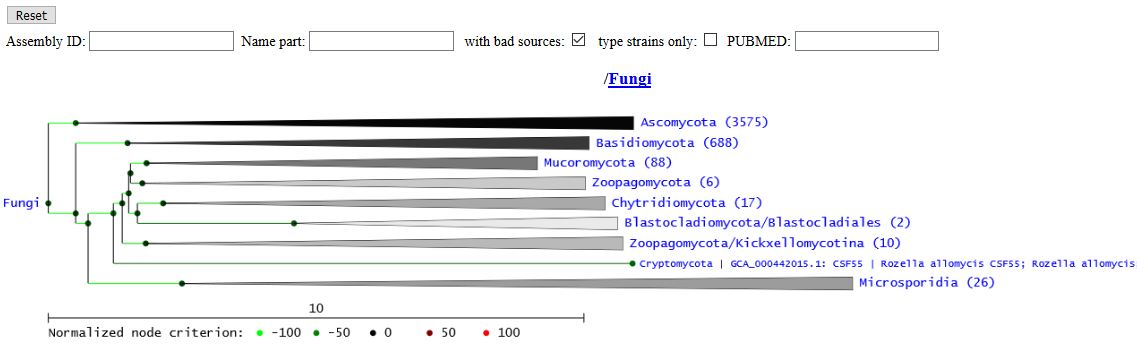
\includegraphics[scale=0.5]{Tree.JPG}
  \caption{Fungal genomes interactive tree}
  \label{fig:Tree}
\end{figure}

The distances are standardized so that~1 is the species barrier,
see Table~\ref{tab:res}.

A part of the tree can be displayed.
Therefore, there are {\em displayed leaves} and {\em final leaves},
as well as {\em displayed root} and {\em global root}.
The final leaves are the tree objects --- genomes or rRNA sequences.

Some nodes have automatically assigned names by the novel method:
the result of the solution of the maximum parsimony problem for the taxons of the objects.

For genomes the names are composed of these items:
\begin{itemize}
  \item automatically assigned taxonomic name (optional) followed by~``$|$'';
  \item ``bad sources'': [SURVEILLANCE], [METAGENOME] or [SINGLE CELL] (optional);
  \item{} [TYPE] (optional);
  \item GenBank assembly accession followed by~``:'';
  \item strain (if it is in GenBank) followed by~``$|$'';
  \item MLST number (only for {\it Escherichia coli} followed by~``$|$'';
  \item serovar (if it is in GenBank) followed by~``$|$'';
  \item semicolon-delimited taxonomic lineage ordered from most specific to most general taxa.
\end{itemize}

For rRNA sequences the names are composed of these items:
\begin{itemize}
  \item automatically assigned taxonomic name (optional) followed by~``$|$'';
  \item RefSeq nucleotide accession, followed by~``:'';
  \item semicolon-delimited taxonomic lineage ordered from most specific to most general taxa.
\end{itemize}

The root is on the left-hand side,
and the displayed leaves are on the right-hand side.
Each displayed leaf should have a name.

If a displayed leaf is an interior node, then its subtree is hidden (collapsed),
and this subtree is shown as a gray triangle where the amount of black color reflects the number of leaves,
followed by the node name and the number of hidden final leaves in parentheses.
The length of the triangle is the average distance to the final leaves weighted by the length of the subtrees.

For each interior node the child subtrees are sorted by the number of final leaves descending,
so that largest subtrees are displayed at the top.
This makes the displayed topology of the trees to be stable among incrementations.

Leaf color reflects the normalized object criterion.
The colors of an interior nodes are derived from the average normalized object criteria of the children.
Arc color reflects the normalized arc error density.

Each interior node is identified by the pair {\tt <top final leaf name>:<bottom final leaf name>},
so that the interior node is the least common ancestor (LCA) of these two final leaves.

Left-clicking on a node opens a Node Information window
containing information on the node and buttons allowing to hide or show ancestors or descendants.
To close the information window, click on any point on the tree.
A single node cannot be displayed, therefore,
hiding ancestors of a leaf node also expands the descendants of the leaf,
and hiding descendants of a root node also expands the ancestors of the root.
Double left-clicking on a leaf or any point to the right of a leaf is the same as hiding ancestors of the leaf,
and double left-clicking on a root or any point on the left margin of the tree is the same as hiding descendants of the root.
Descendants are expanded until named nodes are reached.

The names of final leaves are truncated to~100 characters on the canvas,
but are displayed in full in the Node Information Window.

Objects can be searched by entering the object names (assembly ID or accession for genomes, or RefSeq accessions for rRNA)
or any part of the names of the final leaves.
A colon-delimited list of object identifiers can be entered in the ``Assembly ID'' or ``Nucl. accession'' field.
On pressing the Enter key the found objects are highlighted.
The button ``Zoom in on highlighted'' makes the displayed root to be the LCA of the highlighted objects.
In the pair of numbers $(M/N)$ to the right of a displayed leaf,
$M$~is the number of highlighted objects,
and~$N$ is the total number of objects on the subtree.

If the displayed tree is too large, the ``Make Clusters'' button runs a simple clustering algorithm
which assigns names like ``Cluster N'' to the root nodes of clusters and collapses the clusters,
thus making the displayed tree smaller.



\clearpage
\begin{thebibliography}{9}

\bibitem{Ecoli1K}
Kaleb Abram, Zulema Udaondo, Carissa Bleker, Visanu Wanchai, Trudy M. Wassenaar, Dave W. Ussery,
What can we learn from over 100,000 Escherichia coli genomes?
Jul 19, 2019,
bioRxiv 708131; doi: https://doi.org/10.1101/708131

\bibitem{Agarwala}
Agarwala R. et al.
Database resources of the National Center for Biotechnology Information.
Nucleic Acids Res. 2018 Jan 4;46(D1):D8-D13. doi: 10.1093/nar/gkx1095.

\bibitem{BLAST}
Stephen F. Altschul, Thomas L. Madden, Alejandro A. Schaffer, Jinghui Zhang, Zheng Zhang, Webb Miller, and David J. Lipman (1997),
Gapped BLAST and PSI-BLAST: a new generation of protein database search programs,
Nucleic Acids Res. 25:3389-3402.

\bibitem{maxCongr}
Brover S.,
Principle of a Congruence Maximization of a Phylogenetic Tree to Reference Classifications,
{\it in print}

\bibitem{BUSCO}
Robert M.~Waterhouse, Mathieu Seppey, Felipe A.~Sim�o, Mose Manni, Panagiotis Ioannidis, Guennadi Klioutchnikov, Evgenia V.~Kriventseva, and Evgeny M.~Zdobnov,
BUSCO applications from quality assessments to gene prediction and phylogenomics.
Mol Biol Evol, published online Dec 6, 2017, doi: 10.1093/molbev/msx319

\bibitem{NPHard}
W.H.E.~Day.
Computational complexity of inferring phylogenies from dissimilarity matrices.
Bulletin of Mathematical Biology, 49(4):461-467, 1987.

\bibitem{Felsenstein}
Felsenstein J.
Inferring Phylogenies.
Sunderland, MA: Sinauer Associates, 2003.

\bibitem{Phylip}
Felsenstein J.
1989,
PHYLIP-Phylogeny inference package (version 3.2),
{\it Cladistics} 5:164-166.

\bibitem{HMMer} HMMer. http://hmmer.org/

\bibitem{Prodigal}
Hyatt D, Chen GL, Locascio PF, Land ML, Larimer FW, Hauser LJ.
Prodigal: prokaryotic gene recognition and translation initiation site identification.
BMC Bioinformatics.
2010 Mar 8;11:119. doi: 10.1186/1471-2105-11-119.
PubMed PMID: 20211023; PubMed Central PMCID: PMC2848648.

\bibitem{GenDiscontinuity}
Jain, C., Rodriguez-R, L.M., Phillippy, A.M. et al.
High throughput ANI analysis of 90K prokaryotic genomes reveals clear species boundaries.
Nat Commun 9, 5114 (2018) doi:10.1038/s41467-018-07641-9

\bibitem{GeneMark-ES1}
Lomsadze A., Ter-Hovhannisyan V., Chernoff Y. and Borodovsky M.
"Gene identification in novel eukaryotic genomes by self-training algorithm."
Nucleic Acids Research, 2005, 33: 6494-6506

\bibitem{Spastorianus}
Monerawela C, Bond U.
The hybrid genomes of {\it Saccharomyces pastorianus}: A current perspective.
Yeast. 2018 Jan;35(1):39-50. doi: 10.1002/yea.3250. Epub 2017 Sep 26.
PMID:28787090

\bibitem{GenBank}
Sayers EW, Cavanaugh M, Clark K, Ostell J, Pruitt KD, Karsch-Mizrachi I.
GenBank.
Nucleic Acids Res. 2019 Jan 8;47(D1):D94-D99. doi: 10.1093/nar/gky989. PMID: 30365038; PMCID: PMC6323954.

\bibitem{GTDB}
Parks, D., Chuvochina, M., Waite, D. et al.
A standardized bacterial taxonomy based on genome phylogeny substantially revises the tree of life.
Nat Biotechnol 36, 996-1004 (2018) doi:10.1038/nbt.4229

\bibitem{CheckM}
Parks, D. H., Imelfort, M., Skennerton, C. T., Hugenholtz, P. \& Tyson, G. W.
CheckM: assessing the quality of microbial genomes recovered from isolates, single cells, and metagenomes.
Genome Res. 25, 1043?1055
(2015).

\bibitem{FastTree}
Price MN, Dehal PS, Arkin AP (2010)
FastTree 2 -- Approximately Maximum-Likelihood Trees for Large Alignments.
PLoS ONE 5(3): e9490.
https://doi.org/10.1371/journal.pone.0009490

\bibitem{Silva}
Quast C, Pruesse E, Yilmaz P, Gerken J, Schweer T, Yarza P, Peplies J, Gl�ckner FO (2013)
The SILVA ribosomal RNA gene database project: improved data processing and web-based tools.
Nucl. Acids Res. 41 (D1): D590-D596.

\bibitem{Setubal}
Setubal J., Meidanis J., Introduction to Computational Molecular Biology.
1997.
PWS Publishing Company.

\bibitem{Pfam}
Schaeffer RD, Liao Y, Cheng H, Grishin NV.
ECOD: new developments in the evolutionary classification of domains.
Nucleic Acid Research. 2017; 45(D1):D296-D302.

\bibitem{Rokas}
Shen XX et al.,
Tempo and Mode of Genome Evolution in the Budding Yeast Subphylum.
Cell. 2018 Nov 29;175(6):1533-1545.e20. doi: 10.1016/j.cell.2018.10.023. Epub 2018 Nov 8.

\bibitem{Keppler}
James A. Studier, Karl J. Keppler, A Note on the Neighbor-Joining Algorithm of Saitou and Nei,
Mo. Bio. Evol. 5(6):729-731. 1988

\bibitem{PAUP}
DL Swofford,
Phylogenetic Analysis Using Parsimony, PAUP* 4.0, beta version 4.0 b2,
Sinauer Assoc, Boston, Mass

\bibitem{GeneMark-ES2}
Ter-Hovhannisyan V., Lomsadze A., Chernoff Y. and Borodovsky M.
"Gene prediction in novel fungal genomes using an ab initio algorithm with unsupervised training."
Genome Research, 2008, 18:1979-90

\bibitem{QTree}
Truszkowski, J., Hao, Y. \& Brown, D.G.
Towards a practical O(n logn) phylogeny algorithm.
Algorithms Mol Biol 7, 32 (2012) doi:10.1186/1748-7188-7-32

\bibitem{ASTRAL-MP}
Yin, J., Zhang, C. \& Mirarab, S.
ASTRAL-MP: scaling ASTRAL to very large datasets using randomization and parallelization.
Bioinformatics.
https://doi.org/10.1093/bioinformatics/btz211
(2019).

\bibitem{ASTRAL}
Zhu, Q., Mai, U., Pfeiffer, W. et al.
Phylogenomics of 10,575 genomes reveals evolutionary proximity between domains Bacteria and Archaea.
Nat Commun 10, 5477 (2019).
https://doi.org/10.1038/s41467-019-13443-4



\end{thebibliography}


\bibliographystyle{unsrt}



\end{document}


